\documentclass[11pt]{article}
\usepackage{ifthen}
\usepackage{soul}
\usepackage{fullpage, prettyref}
\usepackage{fancyhdr}
\usepackage{palatino}
\usepackage{graphicx}
\usepackage{marvosym}
\usepackage{ifthen}
\usepackage{algorithm}
\usepackage[noend]{algpseudocode}
\algrenewcomment[1]{\(\triangleright\) {\tiny{#1}}}
\algnewcommand{\LineComment}[1]{\State \(\triangleright\) \emph{\color{blue} #1}}
\newcommand{\Lim}{\lim}
\newcommand{\Exp}{\mathbf{Exp}}

\usepackage{amsmath, amssymb, amsthm}
\usepackage{url}
\usepackage{fullpage, prettyref}
\usepackage{pstricks,pst-node,pst-text}
\usepackage{boxedminipage}
\usepackage{hyperref}
\usepackage{wrapfig}
\usepackage{ifthen}
\usepackage{mdframed}
\usepackage{color,xcolor}
\usepackage{transparent}
\usepackage{enumitem}
\usepackage{varwidth}
\theoremstyle{definition}
\newtheorem{theorem}{Theorem}
\newtheorem{lemma}{Lemma}
\newtheorem{claim}{Claim}
\newtheorem{corollary}{Corollary}
\newtheorem{definition}{Definition}
\newtheorem{proposition}{Proposition}
\newtheorem{fact}{Fact}
\newtheorem{example}{Example}
\newtheorem{exercise}{Problem}
\newtheorem{drill}{Exercise}
\newtheorem{assumption}{Assumption}
\newtheorem{observation}{Observation}

\newcommand{\comment}[1]{\textsl{\small[#1]}\marginpar{\tiny\textsc{To Do!}}}
\newcommand{\ignore}[1]{}

\def\eps{\varepsilon}
\def\bar{\overline}
\def\floor#1{\lfloor {#1} \rfloor}
\def\ceil#1{\lceil {#1} \rceil}
\def\script#1{\mathcal{#1}}

\def\plus{{\tt (+)}}
\def\2plus{{\tt (++)}}
\def\3plus{{\tt (+++)}}
\def\4plus{{\tt (++++)}}
\def\5plus{{\tt (+++++)}}

\def\opt{{\tt opt}}
\def\alg{{\tt alg}}

\def\bv{\mathbf{v}}

\newenvironment{proofof}[1]{\smallskip\noindent{\bf Proof of #1:}}%
{\hspace*{\fill}$\Box$\par}
\setlength{\oddsidemargin}{0pt}
\setlength{\evensidemargin}{0pt}
\setlength{\textwidth}{6.5in}
\setlength{\topmargin}{0in}
\setlength{\textheight}{8.5in}
\newlength{\algobox}
\setlength{\algobox}{6.5in}

\newcommand{\Ex}{\mathbb{E}}
\newcommand{\Var}{\text{Var}}
\newcommand{\hf}{\hat{f}}

\graphicspath{{.}}
\begin{document}
	\begin{center}
		{\bf \Large CS 49/149: 21st Century Algorithms (Fall 2018): Lecture 10}\\ 
		Date: 16th October, 2018 \\
		Topic: Randomized Estimation Algorithms. Median-of-Average trick. \\
		Scribe: Maryam Negahbani \\
		{\em Disclaimer: These notes have not gone through scrutiny and in all probability contain errors. Please email errors to maryam@cs.dartmouth.edu.}
	\end{center}
\hrule height 2pt
\vspace{3ex}
\section{Preliminaries}
\begin{definition}[Discrete Random Variable]
Random variable $X$ is a function defined on some discrete sample space $\Omega$ that takes any $x \in \Omega$ to a value $\Pr[X = x]$ with $0 \leq \Pr[X = x] \leq 1$ such that $\sum\limits_{x \in \Omega} \Pr[X = x] = 1$.
\end{definition}
In this lecture, we use ``random variable'' to refer to a discrete random variable.

\begin{definition}[Independent Random Variables]
Two random variables $X$ and $Y$ are independent if $\Pr[X = x, Y = y] = \Pr[X = x]\Pr[Y = y]$.
\end{definition}

\begin{definition}[Expectation/Mean of a Random Variable] The expected value of a random variable $X$ is denoted by both $\Ex[X]$ and $\mu_x$ and defined as:
\begin{equation*}
   \mu_x = \Ex[x] = \sum\limits_{x \in \Omega} x\Pr[X = x] 
\end{equation*}
\end{definition}
\begin{fact}[Linearity of Expectation]\label{fact:exp}
For any constant $\alpha$ and \textbf{any} two random variables $X$ and $Y$:
\begin{itemize}
    \item $\Ex[\alpha X] = \alpha \Ex[X]$
    \item $\Ex[X + Y] = \Ex[X] + \Ex[Y]$
\end{itemize}
Applying the second formula on any \textbf{finite} set of random variables, say $X_1, X_2,\dots,X_k$ gives:
\begin{equation*}
    \Ex[\sum\limits_{i=1}^k X_i] = \sum\limits_{i=1}^k \Ex[X_i]
\end{equation*}
Note that the $X_i$'s do not need to be independent.
\end{fact}
Next, we define a measure for the expected deviation of a random variable from its expectation. The first thing that comes to mind is to use $X - \Ex[X]$ as $X$'s ``deviation'' from its mean and then take its expectation. But the problem is that $X - \Ex[X]$ is positive for some values of $x \in \Omega$ and negative for some other ones which ``cancel out'' in average and cause $\Ex[X - \Ex[X]] = 0$. The next idea would be to use $|X - \Ex[X]|$ as our deviation but working with absolute values is hard. So we use $(X - \Ex[X])^2$ instead, which leads to the following definition:
\begin{definition}[Variance of a Random Variable]
Variance of a random variable $X$ is denoted by both $\Var[X]$ and $\sigma^2_X$ and defined as:
\begin{equation*}
    \sigma^2_X = \Var[X] = \Ex[(X - \Ex[X])^2] = \Ex[X^2] - \Ex[X]^2
\end{equation*}
\end{definition}
\noindent \textbf{Remark:} $\sigma_X$ is called the standard deviation of $X$.
\begin{fact} \label{fact:var}For any constant $\alpha$, and \textbf{pair-wise independent} random variables $X$ and $Y$ we have:
\begin{itemize}
    \item $\Var[\alpha X] = \alpha^2\Var[X]$
    \item $\Var[X + Y] = \Var[X] + \Var[Y]$
\end{itemize}
\end{fact}
\begin{fact}
$\Var[X] \geq0$ so  $\Ex[X^2] \geq \Ex[X]^2$. 
\end{fact}
Recall that we already knew this by Jensen's inequality since $f(x) = x^2$ is a convex function.
\section{Concentration Inequalities}
Next, we see two inequalities that basically say there is a ``low'' probability that a random variable gets a value ``too far'' from its expectation.
\begin{theorem}[Markov's Inequality]
For any \textbf{non-negative} random variable $X$ and any $t > 0$ we have:
\begin{equation*}
    \Pr[X \geq t] \leq \frac{\Ex[X]}{t}
\end{equation*}
\end{theorem}
\begin{proof}
\begin{align*}
    \Ex[X] = \sum\limits_x x\Pr[X = x] &=  \sum\limits_{x \geq t} x\Pr[X = x] + \sum\limits_{x < t} x\Pr[X = x]\\
                                    &\geq \sum\limits_{x \geq t} x\Pr[X = x] \\
                                    &\geq t\sum\limits_{x \geq t} \Pr[X = x]\\
                                    &= t\Pr[X \geq t]\\
\end{align*}
The first inequality uses the fact that $X$ is non-negative.
\end{proof}
Another way to look at Markov's inequality is by setting $t := \alpha\Ex[X]$ for $\alpha > 0$ which gives:
\begin{equation*}
    \Pr[X \geq \alpha\Ex[X]] \leq \frac{1}{\alpha}
\end{equation*}
Note that this upper-bound is non-trivial only if $\alpha > 1$. So for example, if you wanted to upper-bound the probability of $X \geq \Ex[X]/2$, Markov's inequality is not useful. This brings us to the next inequality:
\begin{theorem}[Chebyshev's Inequality]
For \textbf{any} random variable $X$ and $t>0$ we have:
\begin{equation*}
    \Pr[|X - \Ex[X]| \geq t] \leq \frac{\Var[X]}{t^2}
\end{equation*}
\end{theorem}
\begin{proof}

\begin{equation*}
    \Pr[|X - \Ex[X]| \geq t] = \Pr[(X - \Ex[X])^2 \geq t^2] 
\end{equation*}
As $(X - \Ex[X])^2$ is a non-negative random variable, we can use Markov's inequality to bound the above probability:
\begin{equation*}
    \Pr[(X - \Ex[X])^2 \geq t^2] \leq \frac{\Ex[(X - \Ex[X])^2]}{t^2} = \frac{\Var[X]}{t^2}
\end{equation*}
\end{proof}
Again, to look at Chebyshev's inequality differently, replace $t$ by $\alpha \Var[X]$ for some $\alpha > 0$:
\begin{equation*}
    \Pr[|X - \Ex[X]| \geq \alpha \sqrt{\Var[X]}] \leq \frac{1}{\alpha^2}
\end{equation*}
Qualitatively, if you move $X$ away from $\Ex[X]$ by some factor of $\alpha$, the drop in probability is quadratic with respect to this $\alpha$.

Another benefit of Chebyshev's inequality over Markov's is that in the former, the bound is proportional to $1/\alpha^2$ while in the latter, it is only $1/\alpha$ which means that Chebyshev's bound is tighter with respect to $\alpha$.

\section{Randomized Estimation}
Suppose there is a population of $M$ people and each person has either watched ``Kill Bill'' or not. You are asked to compute the ratio of people that have watched Kill Bill (number of people that have watched it to $M$). Of course, for computing the exact solution, one has to check each person individually and ask if they have watched Kill Bill. However, this can be infeasible if $M$ is large. Then what if you were asked to approximate it? That is, assume the actual solution is $f^*$ and you are supposed to find a $Z$ such that $|Z - f^*| \leq \epsilon$ for some parameter $\epsilon > 0$. This is still not enough, because for small $\epsilon$ and large $M$, you still have to check almost every individual.

Now, what if you are allowed to make ``bad predictions'' sometimes (but not too often). That is, there is a parameter $\delta > 0$ and you could make random predictions as long as $\Pr[|Z - f^*| > \epsilon] \leq \delta$. This $Z$ is a random variable and since it is used for estimation purpose here, we call it a ``random estimator''.

\begin{definition}[$(\epsilon,\delta)$-Estimator]
Random variable $Z$ is an $(\epsilon,\delta)$-estimator for $f^*$ if:
\begin{equation*}
    \Pr[|Z - f^*| \geq \epsilon] \leq \delta
\end{equation*}
\end{definition}
\begin{definition}[Unbiased Estimator]
An estimator $Z$ for $f^*$ is unbiased if $\Ex[Z] = f^*$
\end{definition}
If $Z$ is an unbiased estimator, it gives a correct estimation ``in average''. But we still need to bound the probability of $Z$ giving a far off estimation. Using Chebyshev's inequality, we get:
\begin{equation*}
    \Pr[|Z - f^*| \geq \epsilon] = \Pr[|Z - \Ex[Z]| \geq \epsilon] \leq \frac{\Var[Z]}{\epsilon^2}
\end{equation*}
Thus:
\begin{fact}\label{fact:varbound}
To find an $(\epsilon,\delta)$-estimator, it suffices to find an \textbf{unbiased} estimator $Z$ and show:
\begin{equation*}
    \frac{\Var[Z]}{\epsilon^2} \leq \delta
\end{equation*}
\end{fact}

The following is an example of an unbiased estimator:
\begin{mdframed}[backgroundcolor=blue!05,topline=false,bottomline=false,leftline=false,rightline=false] 
	\underline{\sc Try1}
	\begin{itemize}
		\item Sample an individual uniformly at random
		\item $ Z := \begin{cases} 1& \text{if watched Kill Bill}\\
		0 &\text{otherwise} \end{cases}$
		\item Return $Z$
	\end{itemize}
\end{mdframed}
The $Z$ returned by Try1 is in $\{0,1\}$. These Boolean random variables are called ``indicator random variables'' and in this case, $Z$ is an indicator of watching Kill Bill.
\begin{fact}
If $X \in \{0,1\}$ is indicator of event $S$ we have:
\begin{itemize}
    \item $\Ex[X] = 1\times\Pr[X = 1] + 0\times\Pr[X = 0] = \Pr[S]$
    \item $\Var[X] = \Ex[X^2] - \Ex[X]^2 = \Ex[X] - \Ex[X]^2 = \Pr[S] - \Pr[S]^2 = \Pr[S](1-\Pr[S]) \leq \frac{1}{4}$
\end{itemize}
\end{fact}
\noindent
Thus for our $Z$ we have:
\begin{equation*}
    \Ex[Z] = \Pr[\text{individual has watched Kill Bill}] = \frac{\text{No. of people that watched Kill Bill}}{M} = f^*
\end{equation*}
Which means $Z$ is indeed unbiased. As for the variance:
\begin{equation*}
    \Var[Z] = f^*(1-f^*) \leq \frac{1}{4}
\end{equation*}
Substituting the variance into the equation of fact\eqref{fact:varbound} we get: $1/4 \leq \epsilon^2\delta$ which is totally useless. We would want a ``knob'' on the variance of our estimator, so we could adjust it relative to the parameters we get (a constant variance is not immediately helpful). Nevertheless, in the next section, we will see a general purpose technique for generating a low-variance estimator from an unbiased estimator.
\subsection{The ``Average'' Trick}
\begin{mdframed}[backgroundcolor=blue!05,topline=false,bottomline=false,leftline=false,rightline=false] 
	\underline{\sc Try2}
	(Input: Parameter $k$)
	\begin{itemize}
	
		\item Run Try1 $k$ times to obtain $Z_1,Z_2,\dots,Z_k$
		\item $ Y := \frac{1}{k}\sum_i Z_i$
		\item Return $Y$
	\end{itemize}
\end{mdframed}
By fact\eqref{fact:exp}:
\begin{equation*}
    \Ex[Y] = \frac{1}{k}\sum_i \Ex[Z_i] = f^*
\end{equation*}
And by fact\eqref{fact:var}:
\begin{equation*}
    \Var[Y] = \frac{1}{k^2}\sum_i \Var[Z_i] \leq \frac{1}{4k} \leq \frac{1}{k}
\end{equation*}
So one thing to remember about the average trick is that:

\begin{mdframed}[backgroundcolor=yellow!10,topline=false,bottomline=false,leftline=false,rightline=false] 
		Given an unbiased estimator, the average trick reduces its variance by a factor of $1/k$.
\end{mdframed}

This $k$ is the knob we were looking for. After we substitute $\Var[Y]$ in fact\eqref{fact:varbound} we find the value of $k$ to be:
\begin{mdframed}[backgroundcolor=yellow!10,topline=false,bottomline=false,leftline=false,rightline=false] 
\begin{equation*}
    k = \frac{1}{\epsilon^2\delta}
\end{equation*}
\end{mdframed}

This $Y$ is our first $(\epsilon,\delta)$-estimator. Interestingly, $Y$ is independent of $M$. That is, no matter if your population is small or large, you only need $k$ many samples to give a good estimator. This seems to be counter intuitive but where is the contradiction coming from? Note that, the situation would have been different if we wanted to estimate the \textbf{number} of people that have watched Kill Bill (instead of their ratio). In that case, you would want to find $Y'$ such that for given $\epsilon'$ and $\delta$:
\begin{equation*}
    \Pr[|Y'-f^*M| \geq \epsilon'] \leq \delta \Rightarrow \Pr[|\frac{Y'}{M}-f^*| \geq \frac{\epsilon'}{M}] \leq \delta
\end{equation*}
So if we just substitute $Y'/M$ with $Y$ and replace $\epsilon'/M$ by $\epsilon$ we get our previous problem. But now, the $\epsilon$ depends on $M$ and so is $k$:
\begin{equation*}
    k = \frac{1}{\epsilon^2\delta} = \frac{M^2}{\epsilon'^2\delta}
\end{equation*}
In this case, the number of samples taken by Try2 has a quadratic dependence on the size of the population.
\subsection{The ``Median-of-Average'' Trick}
In this section, we will see another general purpose method for reducing the dependency of the number of samples on $\delta$ from $1/\delta$ to $\log{(1/\delta)}$.

In the last section, we found $Y$ such that $\Pr[|Y - f^*| \geq \epsilon] \leq \delta$ which basically means:
\begin{equation*}
    \Pr[Y \geq f^* + \epsilon \ \text{or} \  y \leq f^* - \epsilon] \leq \delta
\end{equation*}
But what if we only care about bounding $\Pr[Y > f^* + \epsilon]$? By repeating Try2 with $k = 2/\epsilon^2$ for $t$ times independently:
\begin{equation*}
    \Pr[Y_i \geq f^* + \epsilon] \leq \frac{1}{2}, \ \ \forall i\in\{1,2,\dots,t\}
\end{equation*}
What is the probability that \textbf{all of} $Y_1,Y_2\dots,Y_t$ turn out to be bigger than $f^* + \epsilon$? Next, we prove that this probability is small, which means $W := \min_i Y_i$ should be a good estimator.
\begin{align*}
    \Pr[W \geq f^* + \epsilon] &= \Pr[\min_i Y_i \geq f^* + \epsilon] \\&= \Pr[\text{All of $Y_i$'s are} \geq f^* + \epsilon]\\ &= \prod\limits_{i=1}^t \Pr[Y_i \geq f^* + \epsilon] \\&\leq \frac{1}{2^t}
\end{align*}
Thus, to get $\Pr[W \geq f^* + \epsilon] \leq \delta$ we just need to set $t = \log{(1/\delta)}$.
Similarly, for the same $Y_1,Y_2\dots,Y_t$ we can show that if $Q := \max_i Y_i$, then $\Pr[Q \leq f^* - \epsilon] \leq \delta$. So it seems that the good $(\epsilon,\delta)$-estimator for $f^*$ lies somewhere between $W$ and $Q$. The first idea that comes to mind is to use $(W+Q)/2$ as our estimator. But even when both $W$ and $Q$ are good (i.e. $W \leq f^*+ \epsilon$ and $Q \geq f^*- \epsilon$), $(W+Q)/2$ might be far from $f^*$ as shown in the following diagram:
\begin{figure}[h]
\centering
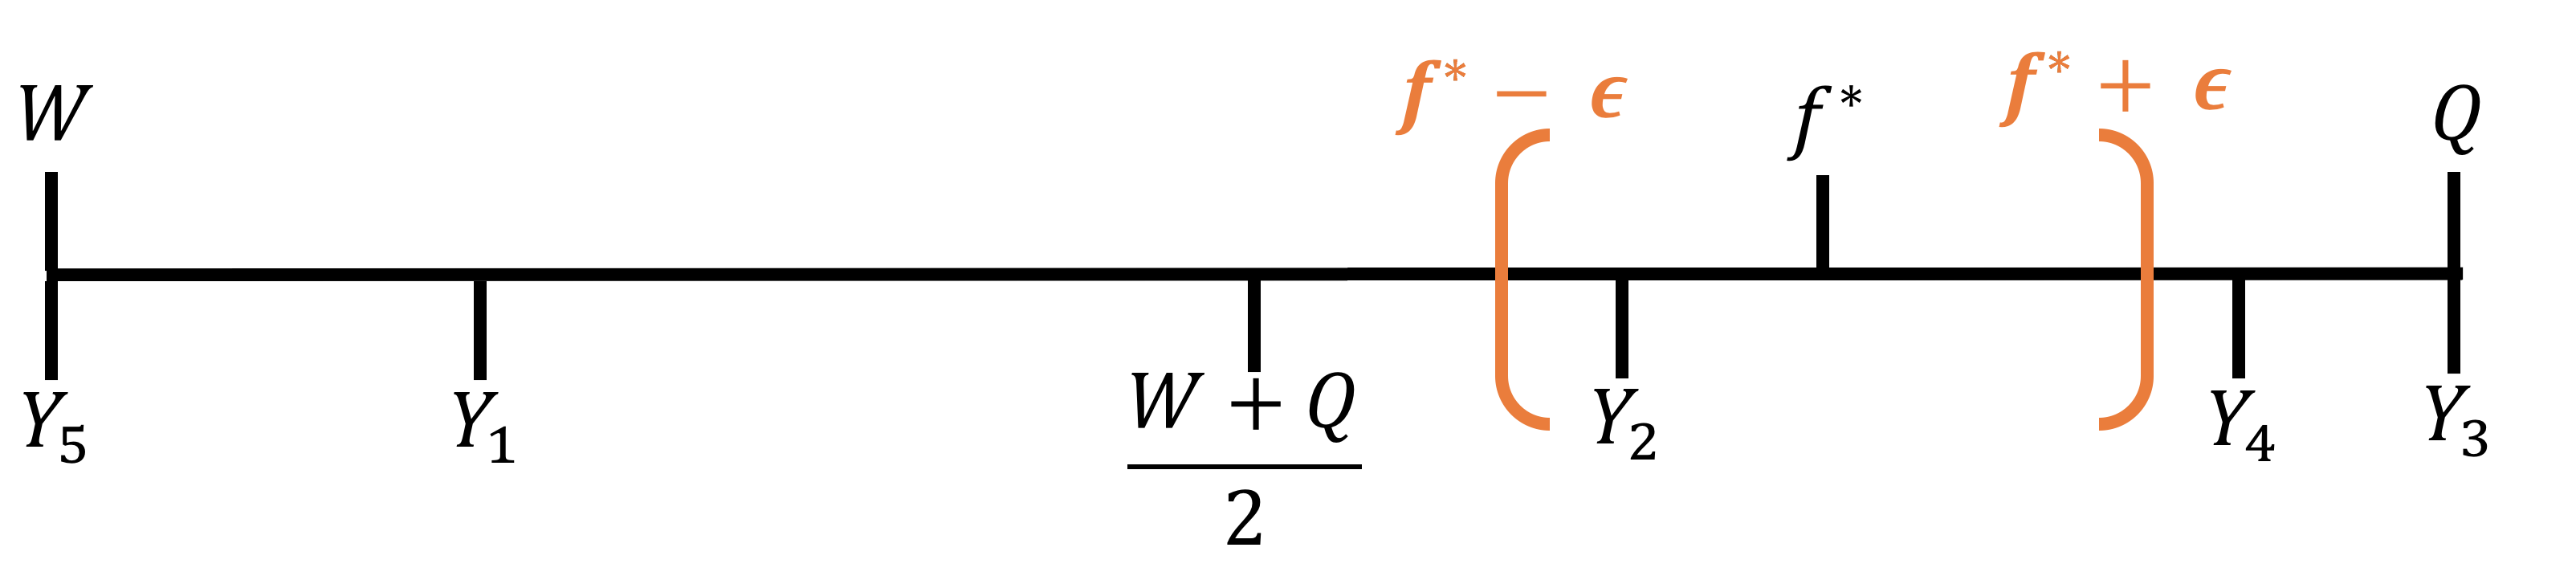
\includegraphics[width=10cm]{pic1.png}
\end{figure}

 However, the picture suggests that the median might be a good estimator. Because for the median to be outside of the $f^*\pm \epsilon$ interval, it must be that at least half of the $Y_i$'s are out of the interval, and the probability of this event is very low.
 \begin{mdframed}[backgroundcolor=blue!05,topline=false,bottomline=false,leftline=false,rightline=false] 
	\underline{\sc Try2.9}
	(Input: Parameter $t$)
	\begin{itemize}
		\item Run Try2 with $k = 2/\epsilon^2$ for $2t+1$ times independently to obtain $Y_1,Y_2,\dots,Y_{2t+1}$
		\item $ \hf := \text{median}(Y_1,Y_2,\dots,Y_{2t+1})$
		\item Return $\hf$
	\end{itemize}
\end{mdframed}
Now we upper-bound $\Pr[\hf \geq f^* + \epsilon]$:
\begin{align*}
    \Pr[\hf \geq f^* + \epsilon] &= \Pr[\text{``some'' $t+1$ many of $Y_i$'s are} \geq f^* + \epsilon]\\
    &= \Pr[\exists S \subset \{1,2,\dots,2t+1\} \ \text{s.t.} \ |S| = t+1 \ \text{and}\ Y_i \geq f^* + \epsilon \ \forall i \in S]
\end{align*}
For any $S \subset \{1,2,\dots,2t+1\}$ of size exactly $t+1$, define $E_S$ to be the event that $Y_i \geq f^* + \epsilon \ $ for all $i \in S$. Since $\Pr[Y_i \geq f^* + \epsilon] \leq \frac{1}{2}$ for all $i \in S$, we have $\Pr[E_S] \leq \frac{1}{2^{t+1}}$.
Assume there are $N$ many of these $S$'s. Then the existence event from the last equality above can be described as the event that $E_{S_i}$ happens for some $i \in \{1,2,\dots,N\}$. By the union bound:
\begin{equation*}
    \Pr[\hf \geq f^* + \epsilon] =  \Pr[E_{S_1}\cup E_{S_2}\cup \dots \cup E_{S_N}]
    \leq \sum\limits_{i=1}^N \Pr[E_{S_i}] \leq \frac{N}{2^{t+1}}
\end{equation*}
Similarly, it can be shown that:
\begin{equation*}
    \Pr[\hf \leq f^* - \epsilon] \leq \frac{N}{2^{t+1}}
\end{equation*}
So overall, the probability that $\hf$ is out of the $f^*\pm \epsilon$ interval is:
\begin{align*}
    \Pr[|\hf - f^*| \geq \epsilon] &= \Pr[\hf \geq f^* + \epsilon \ \text{or} \ \hf \leq f^* - \epsilon]\\
    &\leq \Pr[\hf \geq f^* + \epsilon] + \Pr[\hf \leq f^* - \epsilon]\\
    &\leq \frac{N}{2^t}
\end{align*}
But there is a tiny problem here. $N = \binom{2t+1}{t+1} \approx 4^t$ so our upper-bound becomes trivial. There is an easy fix for this problem: instead of setting $k = 2/\epsilon^2$ let $k = 10/\epsilon^2$.
 \begin{mdframed}[backgroundcolor=blue!05,topline=false,bottomline=false,leftline=false,rightline=false] 
	\underline{\sc Try3}
	(Input: Parameter $t$)
	\begin{itemize}
		\item Run Try2 with $\bf k = 10/\epsilon^2$ for $2t+1$ times independently to obtain $Y_1,Y_2,\dots,Y_{2t+1}$
		\item $ \hf := \text{median}(Y_1,Y_2,\dots,Y_{2t+1})$
		\item Return $\hf$
	\end{itemize}
\end{mdframed}
Now we repeat the previous analysis with this new $k$:
\begin{equation*}
    \Pr[Y_i \geq f^* + \epsilon] \leq \frac{1}{10}, \ \ \forall i\in\{1,2,\dots,2t+1\}
\end{equation*}
\begin{equation*}
    \Pr[\hf \geq f^* + \epsilon]
    \leq \sum\limits_{i=1}^N \Pr[E_{S_i}] \leq \frac{N}{10^{t+1}}
\end{equation*}
\begin{equation*}
    \Pr[|\hf - f^*| \geq \epsilon] \leq \frac{N}{10^t} \approx \frac{4^t}{10^t} = \Big(\frac{2}{5}\Big)^t
\end{equation*}
To get the right hand side to be $\delta$ we set $t$ to be:
\begin{mdframed}[backgroundcolor=yellow!10,topline=false,bottomline=false,leftline=false,rightline=false] 
\begin{equation*}
    t = \log_{\frac{5}{2}}{\frac{1}{\delta}} = O(\log{\frac{1}{\delta}})
\end{equation*}
\end{mdframed}
Putting it all together, the algorithm is: Sample $kt = \frac{10}{\epsilon^2}\log_{\frac{5}{2}}{\frac{1}{\delta}}$ many individuals, divide them into $t$ batches of size $k$ each, compute the average of each batch and return their median.
This median-of-average trick basically says:
\begin{mdframed}[backgroundcolor=yellow!10,topline=false,bottomline=false,leftline=false,rightline=false] 
One can construct an $(\epsilon,\delta)$-estimator given $O(V\frac{1}{\epsilon^2}\log{\frac{1}{\delta}})$ instances of an unbiased estimator with variance $V$.
\end{mdframed}
\end{document}